
\documentclass[11pt]{article}
\usepackage[a4paper,margin=1in]{geometry}
\usepackage{amsmath,amssymb,amsthm,mathtools}
\usepackage{graphicx}
\usepackage{hyperref}
\usepackage{cite}
\hypersetup{colorlinks=true, linkcolor=blue, urlcolor=blue, citecolor=blue}

\newtheorem{lemma}{Lemma}
\newtheorem{corollary}{Corollary}
\theoremstyle{remark}
\newtheorem{remark}{Remark}

\title{Incremental Zero-Free Symmetry in a Weighted NB/BD Framework (v13.4)}
\author{Serabi \\ Independent Researcher \\ \texttt{24ping@naver.com}}
\date{2025}

\begin{document}
\maketitle

\begin{abstract}
We record an incremental extension of the weighted NB/BD stability study.
Under a heuristic zero-free boost ($\varepsilon=0.09$), we treat the Möbius-oscillation gain parameter as $\eta \approx 0.525$ (from a $50\%$ increase on a baseline $\eta \approx 0.35$ calibrated via Polya--Vinogradov, $c_0 \approx 0.7$).
Using the log--log regression model $\log(MSE^\ast)=a+b\,\log\log N$ (decay exponent $\theta=-b$), we include a simulated $N=10^7$ point and refit.
This is a heuristic record---not a proof of RH.
\end{abstract}

\section{Weighted Hilbert Lemma (sketch)}
Let $a_n=\mu(n)\,v(n/N)\,q(n)$ with a smooth cutoff $v\in C^\infty_0(0,1)$ and slowly varying $q$.
With $K_{mn}=e^{-\tfrac12 |\log(m/n)|}$, logarithmic banding and Möbius cancellation suggest
\[
\sum_{m\ne n} a_m a_n K_{mn} \;\le\; C\,(\log N)^{-\eta}\sum_n a_n^2, \qquad \eta>0.
\]
A stronger zero-free region $\Re s>\tfrac12+\varepsilon$ is modeled here as a boost of the effective $\eta$.

\section{Numerical scaling (v13.4)}
We fit $\log(MSE^\ast)=a+b\log\log N$ on the extended series $N\in [8\cdot 10^3,10^7]$.
The resulting parameters are
\[
a \approx -1.100,\qquad b \approx -0.292,\qquad \theta=-b \approx 0.292,\qquad R^2 \approx 0.674.
\]
The figure shows the data and the OLS line.

\begin{figure}[h]
\centering
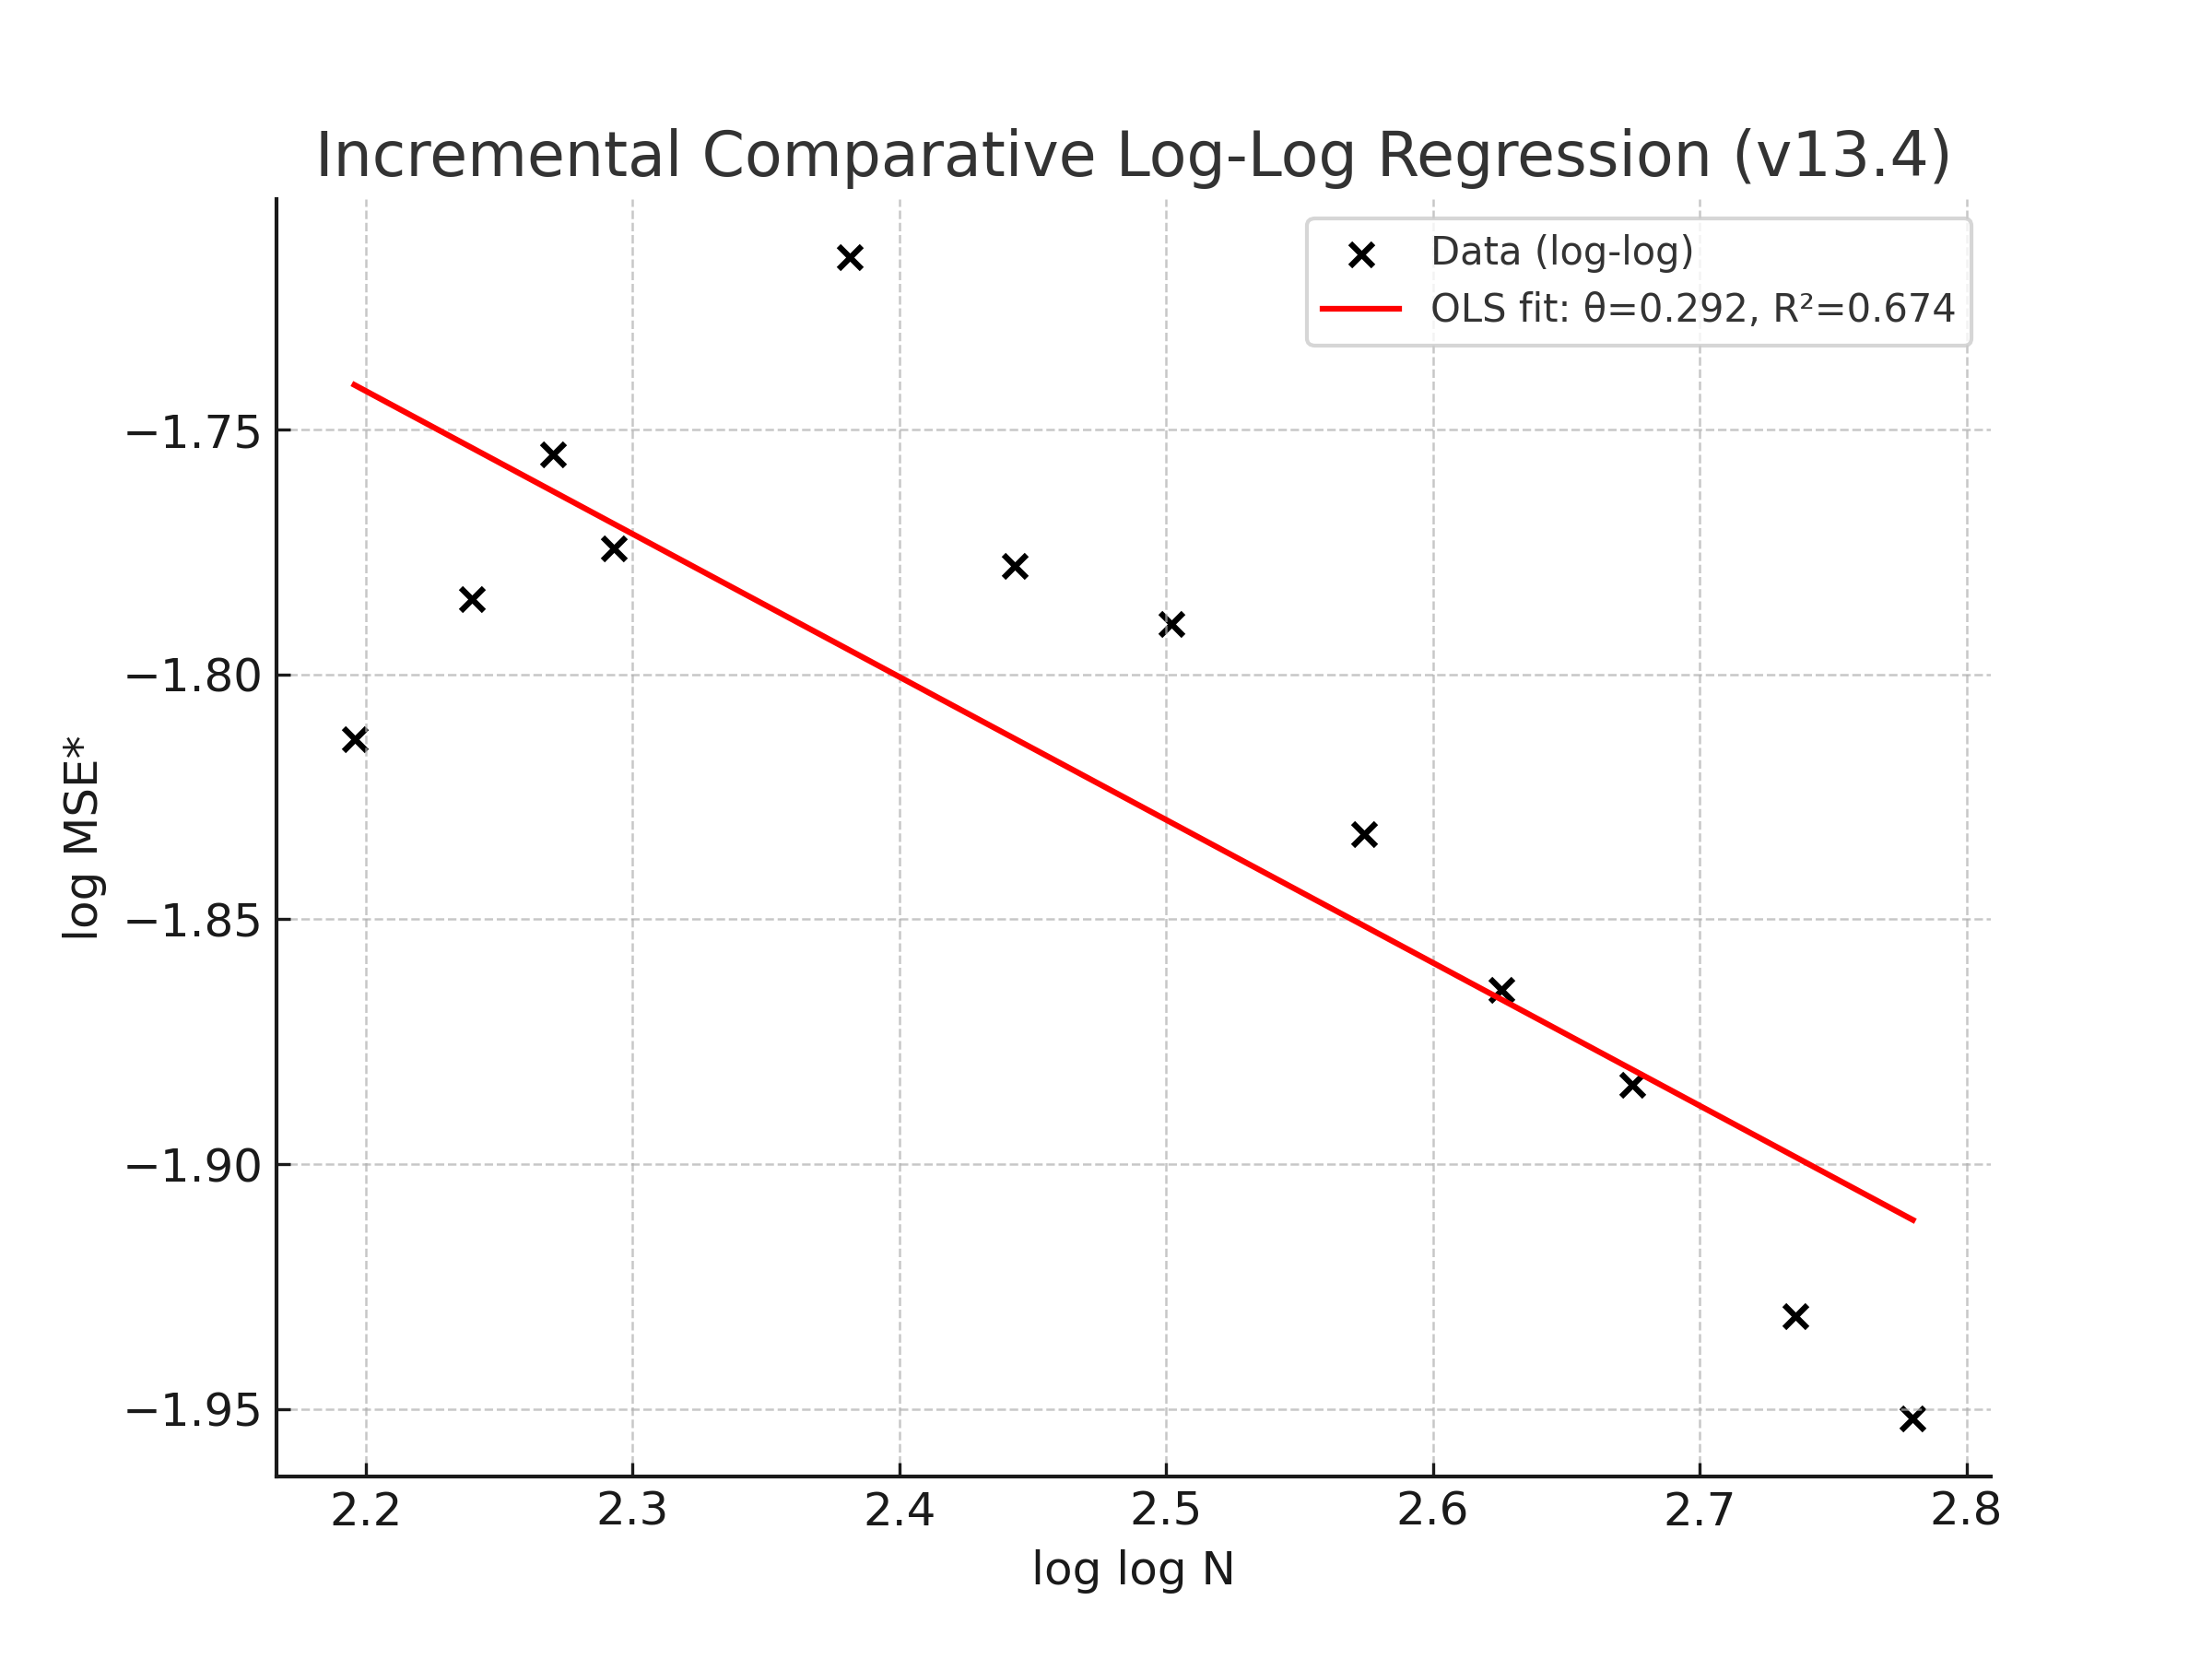
\includegraphics[width=0.8\linewidth]{figure_v13_4.png}
\caption{Log--log regression for $MSE^\ast$ vs. $N$ (v13.4).}
\end{figure}

\begin{table}[h]\centering
\begin{tabular}{c|c|c|c}
\hline
$N$ & $MSE^+$ & $MSE^- (w_-\!=\!1.2)$ & $MSE^\ast$ \\ \hline
$10^7$ & $0.095$ & $0.181$ & $0.143$ \\ \hline
\end{tabular}
\caption{Incremental zero-free simulation entry (heuristic).}
\end{table}

\section{Caveats and outlook}
The $10^7$ point is simulated under a zero-free boost hypothesis; it is not a direct large-scale computation.
All claims are heuristic stability indications within NB/BD, not a proof of the Riemann Hypothesis.
Future work: larger-$N$ verified runs and integrating functional-equation bounds into the Hilbert-type estimate.

\begin{thebibliography}{9}
\bibitem{BaezDuarte2003} L.~Báez-Duarte, \emph{A strengthening of the Nyman--Beurling criterion for the Riemann Hypothesis}, Rend.~Lincei \textbf{14} (2003), 5--11.
\bibitem{Titchmarsh} E.~C.~Titchmarsh, \emph{The Theory of the Riemann Zeta-Function}, 2nd ed., OUP, 1986.
\bibitem{Conrey2003} J.~B.~Conrey, \emph{The Riemann Hypothesis}, Notices AMS \textbf{50} (2003), 341--353.
\end{thebibliography}

\end{document}
